%% Manuscript prepared for Applied Energy (Elsevier, elsarticle class).
%% Build: pdflatex main && bibtex main && pdflatex main && pdflatex main
\documentclass[preprint,12pt]{elsarticle}

\usepackage[T1]{fontenc}
\usepackage{lmodern}
\usepackage{amsmath,amssymb}
\usepackage{graphicx}
\usepackage{booktabs}
\usepackage{xcolor}
\usepackage[hidelinks]{hyperref}
\hypersetup{hypertexnames=false}
\usepackage{lineno}
\usepackage{microtype}
\usepackage{caption}
\captionsetup{font=small,labelfont=bf}

\newcommand{\eg}{e.g.,\ }
\newcommand{\ie}{i.e.,\ }
\newcommand{\pd}{\mathrm{PD}}
\DeclareMathOperator*{\argmin}{arg\,min}
\DeclareMathOperator{\med}{med}
\DeclareMathOperator{\asinh}{asinh}

\journal{Applied Energy}

\begin{document}

\begin{frontmatter}

\title{Dual-Field Electricity Price Forecasting with Predispatch}

%% Author details to be completed by the author before submission.
\author[inst1]{zl\corref{cor1}}
\ead{[e-mail]}
\cortext[cor1]{Corresponding author.}
\affiliation[inst1]{organization={[Affiliation]},
            city={[City]},
            country={[Country]}}

\begin{abstract}
Wholesale electricity prices combine a changing level with scarcity spikes and negative-price troughs. We adapt the trend--event structure of DualTimesField to rolling 24-hour forecasting using detected historical events, a linear base, and point-in-time market-operator forecasts. Experiments cover three regions of the Australian National Electricity Market, with 17{,}521 hourly origins per region in 2023--2024. On a single fit to 2015--2021, the fields worsen mean absolute error (MAE) relative to the same linear base, although they improve its approximate continuous ranked probability score (CRPS). With quarterly refits and AEMO predispatch inputs, the fields improve both metrics when pooled across regions; point-forecast gains are not uniform across regions. A shared per-hour calibrator and a validation-selected lower bound further reduce MAE. The final model achieves a three-region mean MAE of 36.6~AUD/MWh, below PatchTST, DLinear and a linear baseline (pooled Diebold--Mariano $p<0.01$), but above XGBoost at 35.5. Its negative-price CRPS is lower than all five main-table comparators ($p<0.001$). The lower bound trades a small deterioration in negative-price scores for better overall MAE. These results identify the conditions and limits of the decomposition's forecasting value.
\end{abstract}

\begin{highlights}
\item A trend--event dual-field model is adapted from reconstruction to price forecasting.
\item Static-fit fields worsen MAE but improve CRPS relative to the same linear base.
\item Quarterly refits and predispatch yield pooled gains, with regional differences.
\item Negative-price scores improve over all five main-table comparators.
\item A validation-selected lower bound trades tail accuracy for lower overall MAE.
\end{highlights}

\begin{keyword}
Electricity price forecasting \sep Probabilistic forecasting \sep Time-series decomposition \sep Negative prices \sep National Electricity Market \sep Predispatch
\end{keyword}

\end{frontmatter}

\linenumbers

%% ---------------------------------------------------------------------------
\section{Introduction}
\label{sec:introduction}

Short-term electricity price forecasts drive bidding, storage dispatch, demand response and hedging decisions \citep{weron2014electricity,hong2020energy}. In markets with a fast-growing share of wind and solar generation, these forecasts have become harder. Prices still follow a daily and seasonal level, but they are increasingly punctuated by events: scarcity spikes when supply margins tighten and negative-price troughs when renewable output exceeds demand. In the Australian National Electricity Market (NEM), the share of hours with negative prices in Queensland rose from 1.6\% in 2015--2021 to 13.2\% in 2023--2024 (Section~\ref{sec:data}). A forecaster that treats these events as noise around a level misses exactly the hours in which storage and flexible demand earn or lose most.

Separating a series into a continuous trend and discrete events is therefore an attractive structural prior. Classical decompositions and their neural successors \citep{wu2021autoformer,oreshkin2020nbeats,zeng2023transformers} split trend from seasonality; DualTimesField \citep{zhang2026dualtimesfield} goes further and represents a series as a continuous trend field (CTF), an implicit neural representation in continuous time \citep{sitzmann2020implicit,tancik2020fourier}, plus a discrete event field (DGF) of localized atoms. It was designed for reconstruction and interpolation. Whether such a representation helps forecasting is not obvious: describing the past more faithfully does not by itself add information about the future, and a richer description of a past regime can overfit it.

This paper studies that question for rolling 24-hour price forecasting in three NEM regions, under a same-data protocol in which every compared model receives the same underlying inputs, the same training periods and the same evaluation. Our findings are sequential, and the paper follows them:

\begin{enumerate}
\item \emph{Transplanted, the dual field does not separate events.} The CTF absorbs spikes and the DGF collapses. Detecting events explicitly, as the largest departures from the window median, restores the separation (\ref{app:static}).
\item \emph{Separation alone does not improve point accuracy.} On a single fit to 2015--2021, a linear model on the same inputs has lower MAE than the dual-field model. Adding the fields to the same linear base raises MAE but lowers CRPS (Section~\ref{sec:when}). Lower training loss and higher validation MAE are consistent with overfitting to the training-period price regime.
\item \emph{Recalibration and market-operator information yield pooled gains.} Motivated by the frequent recalibration used in electricity price forecasting \citep{lago2021forecasting}, we refit every model before each test quarter. AEMO's predispatch combines current offers, constraints and demand forecasts, and lowers every model's three-region mean MAE. With these inputs and refits, the dual fields improve pooled MAE and CRPS over the same linear base; raw-price MAE nevertheless worsens in QLD1.
\item \emph{Diagnosis-driven corrections.} A per-region analysis of the errors that remain against the strongest competitor locates them in negative-price hours, where linear heads over-extrapolate in the transformed target space. A shared per-hour calibrator and a price floor chosen on validation data address this and are each significant.
\end{enumerate}

The final model has lower MAE than PatchTST \citep{nie2023time}, DLinear \citep{zeng2023transformers} and a linear model, and lower negative-price CRPS and lower-tail pinball loss than the five main-table comparators. XGBoost \citep{chen2016xgboost} with the same inputs and refits remains more accurate on overall MAE and CRPS. The final model is not the best of all development variants on negative-price scores: omitting its lower bound improves those scores but worsens overall MAE. Beyond the model, the study shows why a structured forecaster should be evaluated against strong same-input baselines and under its intended recalibration regime.

The rest of the paper is organized as follows. Section~\ref{sec:related} reviews related work. Section~\ref{sec:data} describes the data and the forecasting task, Section~\ref{sec:method} the model, and Section~\ref{sec:setup} the experimental protocol. Section~\ref{sec:results} reports the results, Section~\ref{sec:discussion} discusses them, and Section~\ref{sec:conclusion} concludes.

%% ---------------------------------------------------------------------------
\section{Related work}
\label{sec:related}

\paragraph{Electricity price forecasting} Reviews by \citet{weron2014electricity} and \citet{nowotarski2018recent} survey point and probabilistic electricity price forecasting. \citet{lago2021forecasting} established an open benchmark and best practices, among them daily recalibration on a rolling window, variance-stabilizing transformations \citep{uniejewski2018variance}, and comparison against well-specified linear (LEAR) and neural baselines with Diebold--Mariano tests \citep{diebold1995comparing}. High-dimensional linear models \citep{ziel2018day} and distributional neural networks \citep{marcjasz2023distributional} are strong references. We follow these practices: an asinh transformation, rolling recalibration, same-input baselines, and significance tests.

\paragraph{Deep time-series forecasting and decomposition} Transformer forecasters such as Informer \citep{zhou2021informer}, Autoformer \citep{wu2021autoformer}, PatchTST \citep{nie2023time} and iTransformer \citep{liu2024itransformer}, recurrent models \citep{hochreiter1997long,cho2014learning} and DeepAR \citep{salinas2020deepar} have been widely applied. \citet{zeng2023transformers} showed that a decomposed linear model (DLinear) is competitive with many of them. N-BEATS \citep{oreshkin2020nbeats} and Autoformer use trend and seasonal decompositions inside the network; hybrid models combine a linear component with a nonlinear residual \citep{zhang2003time}. DualTimesField \citep{zhang2026dualtimesfield} represents trend and events as continuous-time fields for reconstruction. Our model adds dual fields as a residual to a linear base, and asks when this structure pays off in forecasting.

\paragraph{Exogenous information and strong tabular baselines} Fundamental forecasts of load, renewable output and capacity are established inputs in electricity price forecasting \citep{weron2014electricity,lago2021forecasting}. Recent work adds text: \citet{chen2026reprice} introduce RE-Price, which combines structured news extraction, cross-modal attention and a QLoRA-adapted Qwen3-4B backbone. Monte Carlo dropout under standard and tail-aware prompts generates scenarios, which are smoothed with adaptive Gamma kernels. Their study uses the same three NEM regions and the 2015--2024 period, with a chronological 70/10/20 split and 72-hour inputs for 24-hour forecasts. However, its inputs include WattClarity news and temperature-forecast proxies constructed from noisy observations, whereas our main setting uses numerical market-operator forecasts with quarterly refits. The information sets and evaluation protocols therefore differ; RE-Price is related work, not a reproduced same-data competitor, and its published errors are not directly comparable with ours. The strong performance of gradient-boosted trees on tabular benchmarks \citep{grinsztajn2022tree} motivates including XGBoost alongside neural baselines.

%% ---------------------------------------------------------------------------
\section{Data and forecasting task}
\label{sec:data}

\paragraph{Market and prices} We use hourly regional reference prices (RRP) and operational demand for New South Wales (NSW1), Queensland (QLD1) and Tasmania (TAS1) from AEMO's aggregated price and demand data \citep{aemo2025priceanddemand}, 1 January 2015 to 31 December 2024 in market time (AEST), with half-hourly records averaged to hours. Table~\ref{tab:data} summarizes the series. The test period, 2023--2024, differs markedly from 2015--2021: negative prices are four to eight times more frequent, spikes above 300~AUD/MWh are more frequent in NSW1 and QLD1, and 2022, the energy-crisis year that separates them, has a much higher level.

\begin{table}[t]
\centering
\caption{Hourly regional reference prices (AUD/MWh) by period. Neg.: share of hours below zero; $>300$: share of hours above 300~AUD/MWh.}
\label{tab:data}
\small
\begin{tabular}{llrrrrr}
\toprule
Region & Period & Mean & Median & Std. dev. & Neg. & $>300$ \\
\midrule
NSW1 & 2015--2021 & 70.5 & 58.0 & 164.9 & 0.37\% & 0.25\% \\
     & 2022       & 182.7 & 135.4 & 215.3 & 2.61\% & 14.79\% \\
     & 2023--2024 & 113.5 & 82.7 & 408.8 & 6.20\% & 1.75\% \\
\midrule
QLD1 & 2015--2021 & 70.9 & 55.2 & 202.5 & 1.63\% & 0.68\% \\
     & 2022       & 205.1 & 139.9 & 456.2 & 4.05\% & 15.73\% \\
     & 2023--2024 & 101.1 & 81.3 & 289.2 & 13.21\% & 1.85\% \\
\midrule
TAS1 & 2015--2021 & 69.4 & 57.6 & 68.7 & 2.53\% & 0.43\% \\
     & 2022       & 147.0 & 104.9 & 285.3 & 1.82\% & 8.57\% \\
     & 2023--2024 & 75.8 & 60.3 & 168.2 & 7.36\% & 0.50\% \\
\bottomrule
\end{tabular}
\end{table}

\paragraph{Forecasting task} Let $p_t$ denote the price for the delivery hour starting at $t$. At origin $t$, the target is $(p_t,\dots,p_{t+23})$, using observations from hours $t-72,\dots,t-1$ and exogenous information published by $t$. The observation for hour $t-1$ becomes available at $t$; no target-hour observation enters the history. We index the 24 forecast outputs by $h=0,\dots,23$. Origins advance hourly, giving 17{,}521 complete test windows per region. This is a rolling 24-hour task, distinct from a fixed-origin day-ahead auction forecast.

\paragraph{Known inputs} Four groups of forward-looking information enter every model, each as published at the origin:
\begin{itemize}
\item \emph{Calendar}: hour of day, day of week and day of year (sine and cosine), month, weekend flag and a standardized year.
\item \emph{PD PASA}: AEMO's pre-dispatch projected assessment of system adequacy \citep{aemo2025mmsdm}, from which we take maximum spare capacity and net load (50\%-probability demand minus semi-scheduled wind and solar availability) for each forecast hour, from the latest run published by the origin, with the short-term PASA run filling hours beyond its horizon.
\item \emph{Gas}: the logarithm of the seven-day trailing mean of the Victorian declared wholesale gas market price \citep{aemo2025dwgm}, using only gas days ended before the origin.
\item \emph{Predispatch}: AEMO's predispatch re-solves the market dispatch every 30 minutes with current offers, constraints and demand forecasts. Its horizon extends to the end of the trading day for which bid prices have closed, and expands to include the next trading day at 12:30 AEST \citep{aemo2026predispatch}. We obtain regional price and quantity forecasts from the MMSDM archive \citep{aemo2025mmsdm}. For each origin we take the latest run whose rows were all published by then and keep the forecast price, total demand, available generation and net interchange for each hour. Runs published between about 04:00 and 12:30 end before the 24th forecast hour; uncovered hours repeat the last covered hour and are flagged (93\% of hours are covered). The archive has no run history for October 2022, whose origins are marked uncovered and filled with training-period medians.
\end{itemize}
Used directly as a forecast, the predispatch price has a test MAE of 147.5, 153.3 and 69.4~AUD/MWh in NSW1, QLD1 and TAS1, inflated by spikes that do not materialize, but a median absolute error of only 17--20~AUD/MWh: it is informative but must be calibrated.

\paragraph{Price treatments} We evaluate on raw prices and, as a robustness check that limits the weight of a few extreme hours in absolute-error metrics, on prices capped at 650~AUD/MWh, with the cap applied to the price series used as target and as history, in training and in scoring.

%% ---------------------------------------------------------------------------
\section{Method}
\label{sec:method}

Fig.~\ref{fig:framework} gives an overview. The forecast is the sum of a linear base on all inputs, a dual-field residual built from a trend--event decomposition of the history, and a calibration term, followed by a price floor. Every component is refit before each test quarter.

\begin{figure}[t]
\centering
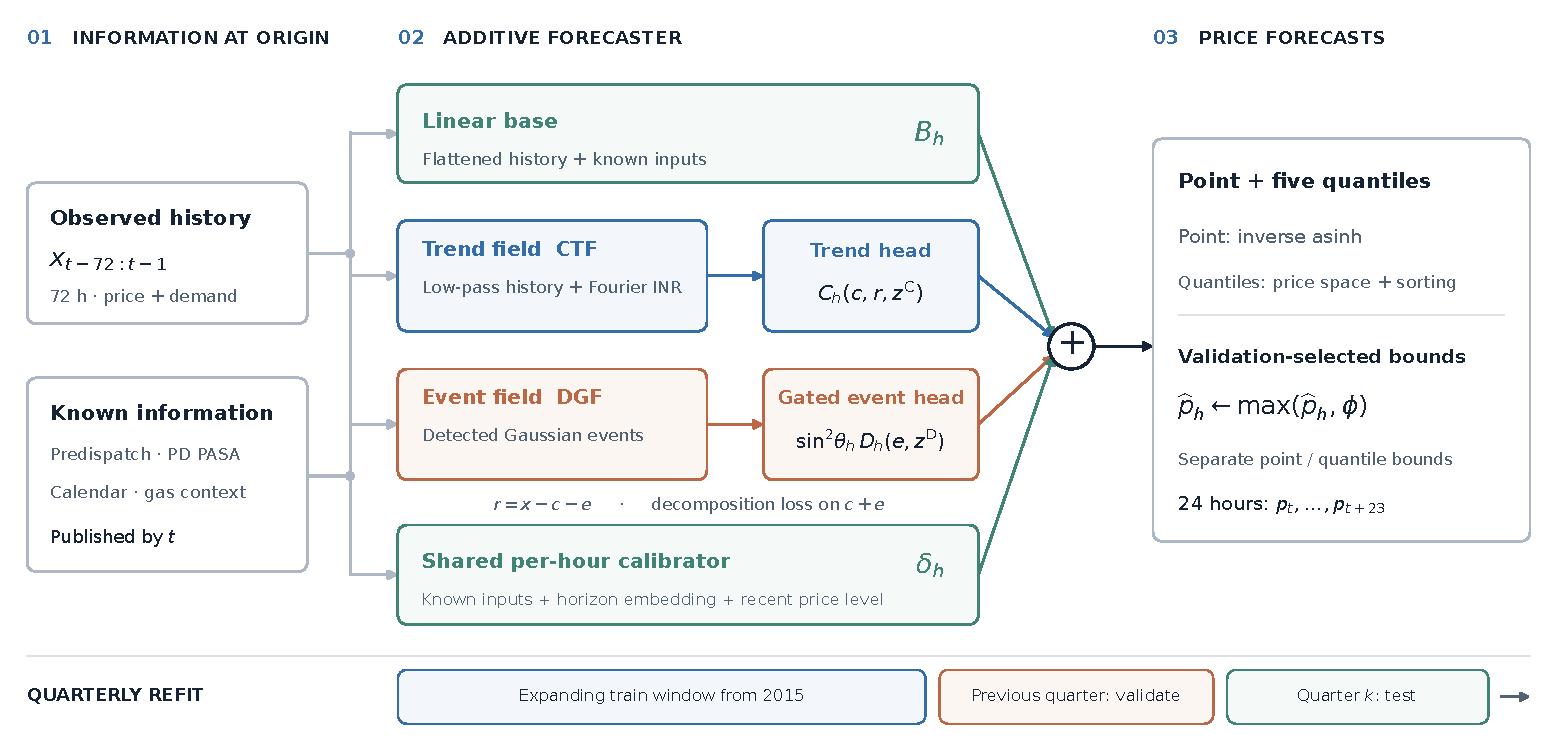
\includegraphics[width=\textwidth]{figures/framework.pdf}
\caption{Dual-field forecasting architecture. (a) The 72-hour price and demand history $x$ and information $z$ published by origin $t$ supply the model inputs; matching tags indicate the context used by each head. (b) The CTF reads low-pass full history and Fourier time features, while the DGF detects localized price events directly from history. Their forecast heads, a linear base and a shared per-hour calibrator contribute additively; the CTF head also reads the remainder $r=x-c-e$, and the event contribution is gated. (c) Point outputs are inverse-transformed, price-space quantiles are sorted, and separate validation-selected lower bounds are applied. The solid point forecast need not equal the dashed median; shaded bands denote the central 80\% and 90\% quantile intervals. All curves are illustrative, not recorded predictions. Exact feature routing and quantile-specific gates are specified in Section~\ref{sec:method}.}
\label{fig:framework}
\end{figure}

\subsection{Target transformation}
Prices are mapped by the area hyperbolic sine with median and median-absolute-deviation scaling \citep{uniejewski2018variance},
\begin{equation}
y = \asinh\!\left(\frac{p-\mu}{\sigma}\right),\qquad \mu=\med(p^{\mathrm{train}}),\quad \sigma=\frac{\med|p^{\mathrm{train}}-\mu|}{0.6745},
\end{equation}
and standardized with training statistics. The point forecast is produced in this space and mapped back by the inverse transform. The quantile forecasts are produced directly in standardized price space, which keeps their spread in the units on which they are scored.

\subsection{Dual-field decomposition of the history}
Let $x\in\mathbb{R}^{72\times 2}$ be the standardized history of transformed price and demand, indexed by $\tau=1,\dots,72$.

\paragraph{Event field (DGF)} Events are detected in the price channel $x^{(1)}$ relative to a robust level. With departures $d_\tau=x^{(1)}_\tau-\med_\tau x^{(1)}_\tau$, we select $K=8$ positions $c_1,\dots,c_K$ greedily by largest $|d_\tau|$, suppressing positions closer than three hours to an already selected one. Each event keeps its departure, soft-thresholded by a learned level $\kappa>0$, and becomes a Gaussian bump of learned width $w$:
\begin{equation}
e(\tau)=\sum_{k=1}^{K} a_k \exp\!\left(-\frac{(\tau-c_k)^2}{2w^2}\right),\qquad a_k=\operatorname{sign}(d_{c_k})\max\!\left(|d_{c_k}|-\kappa,\,0\right).
\end{equation}
Event positions are determined by the history, while the threshold and width remain learned parameters ($w=\mathrm{softplus}(w_0)+0.25$ hours). The event signal is nonzero only in the price channel; its demand channel is zero. This constrains the decomposition more directly than globally learned event positions (\ref{app:static}); it does not impose a fixed event signal throughout training.

\paragraph{Trend field (CTF)} The CTF is a Fourier-feature implicit neural representation \citep{tancik2020fourier,zhang2026dualtimesfield}. With normalized time $\tau'\in[0,1]$, learned band-limited frequencies $b_j=\omega_{\max}\,\mathrm{sigmoid}(\beta_j)$, $j=1,\dots,16$, and a low-pass filtered copy $\tilde x_\tau$ of the history,
\begin{equation}
\gamma(\tau')=\big[\cos 2\pi b_j\tau',\ \sin 2\pi b_j\tau'\big]_{j=1}^{16},\qquad c(\tau)=f_\theta\big(\gamma(\tau'),\,\tilde x_\tau\big),
\end{equation}
where $f_\theta$ is a small multilayer perceptron. The CTF receives the low-pass filtered full history, not an event-subtracted input. The decomposition loss $\mathcal{L}_{\mathrm{dec}}=\|c+e-x\|_2^2/|x|$ encourages it to account for the signal not represented by the events, and $r=x-c-e$ is the remainder. The net-load input to its forecast head is standardized on training data, with logarithmic compression beyond the training 0.5\% and 99.5\% quantiles.

\subsection{Forecast heads, linear base and fusion}
For each of the 24 forecast hours $h$, linear heads map field features to a point forecast in transformed space and to quantiles at the levels 0.05, 0.10, 0.50, 0.90 and 0.95 in price space:
\begin{itemize}
\item \emph{CTF heads} read the trend $c$, the remainder $r$, the calendar, the gas price and the PD PASA net load: the level and its fundamental drivers.
\item \emph{DGF heads} read the event field $e$, the calendar, the PD PASA spare capacity and the predispatch inputs; the DGF quantile head also reads the shortfalls of spare capacity below its training 1\%, 5\% and 10\% quantiles, a piecewise-linear scarcity response.
\end{itemize}
The two are fused by an additive trigonometric gate, $\hat y^{\mathrm{F}}_h=\hat y^{\mathrm{C}}_h+\sin^2(\theta_h)\,\hat y^{\mathrm{D}}_h$, with $\theta_h=\tfrac{\pi}{2}\,\mathrm{sigmoid}(g_h)$ and $g_h$ linear in the fields, the calendar and the DGF inputs; each quantile level has its own affine rescaling of $g_h$, so tail quantiles can draw on the event field more than the median.

The \emph{linear base} $\hat y^{\mathrm{B}}$ is one linear map from the standardized, undecomposed history and all known inputs to the 24 point and quantile outputs. The fused field forecast is added to it as a residual, so the fields only need to model what a linear function of the inputs cannot.

\paragraph{Calibrator} A single perceptron with two 32-unit hidden layers and GELU activations, shared by all forecast hours, reads hour $h$'s known inputs (predispatch, PD PASA, calendar), a learned four-dimensional horizon embedding and two transformed-price summaries (last observed value and 24-hour mean), and outputs additive corrections $\delta_h$ to the point and quantile forecasts. Its output layer is initialized at zero. It lets the model learn a nonlinear response to predispatch, for example that high predispatch prices are often not realized. The point forecast before inverse transformation and the lower bound is
\begin{equation}
\hat y_h=\hat y^{\mathrm{B}}_h+\hat y^{\mathrm{F}}_h+\delta_h .
\end{equation}

\paragraph{Training} The recorded training and checkpoint-selection loss is
\begin{equation}
\mathcal{L}=\underbrace{\tfrac{1}{24}\textstyle\sum_h(\hat y_h-y_h)^2}_{\text{point}}+\underbrace{\tfrac{1}{24\cdot5}\textstyle\sum_{h,q}\rho_q\!\left(\tilde p_h-\hat{\tilde p}_{h,q}\right)}_{\text{quantiles}}+\mathcal{L}_{\mathrm{dec}}+\lambda_s\mathcal{L}_{\mathrm{smooth}}+\lambda_g\mathcal{L}_{\mathrm{sparse}},
\end{equation}
where $\rho_q$ is the pinball loss \citep{koenker1978regression}, $\tilde p$ is the standardized price, and $\mathcal{L}_{\mathrm{smooth}}$ penalizes squared first differences of the CTF. The retained implementation computes $\mathcal{L}_{\mathrm{sparse}}=\bar z+10\max(\bar z-0.3,0)$, where $z_k=\mathbf{1}[a_k\ne0]$ and $\bar z$ is the batch mean ($\lambda_s=\lambda_g=10^{-3}$). This hard indicator has no gradient: the sparsity term contributes to the reported loss and checkpoint selection, but does not directly regularize parameter updates. Event sparsity instead results from selecting at most eight positions and soft-thresholding their amplitudes; the threshold and width receive gradients through the reconstruction and forecasting terms. We use AdamW with learning rate $3\times10^{-4}$, weight decay $10^{-4}$, batch size 128 and 30 epochs, and keep the epoch with the lowest recorded validation loss. The model has 277{,}747 parameters. Quantiles are sorted after field fusion, addition of the base, and calibration to prevent crossings.

\subsection{Price floor}
The fitted linear heads can extrapolate to very low prices after the inverse asinh transform (Section~\ref{sec:diagnosis}). We apply an empirical lower bound, $\hat p_h\leftarrow\max(\hat p_h,\phi)$; this is a forecast calibration choice, not the NEM's regulatory market price floor or a physical bound on negative prices. For each refit and region, $\phi$ is chosen on that refit's validation quarter from $\{$none$\}\cup\{\min(Q_\alpha(p^{\mathrm{train}}),0):\alpha\in\{0.05,0.1,0.2,0.5,1\}\%\}$. The training-price sample here pools the training target windows. Point and quantile lower bounds are selected separately by mean validation MAE and CRPS over the three seeds, respectively. No test-quarter prices are used to select the numerical bound. Its effect on negative-price scores is reported separately from its overall MAE gain.

\subsection{Quarterly recalibration}
Before each of the eight test quarters $k$ (2023Q1 to 2024Q4), every model is refit on data from January 2015 to three months before the quarter, selects its checkpoint on those three months, and forecasts the origins of the quarter. Forecasts of the eight quarters together cover exactly the 17{,}521 test origins of each region. Transformations, standardizations and quantile knots are re-estimated on each refit's training data.

%% ---------------------------------------------------------------------------
\section{Experimental setup}
\label{sec:setup}

\paragraph{Baselines} All baselines receive the same history and known inputs, including predispatch, and are refit on the same quarterly schedule.
\begin{itemize}
\item \emph{XGBoost} \citep{chen2016xgboost}: one multi-quantile model per forecast hour on the flattened history, gas price and that hour's calendar and known inputs (depth 6, learning rate 0.05, subsampling 0.8, up to 2{,}000 rounds with early stopping on validation); the median is the point forecast.
\item \emph{PatchTST} \citep{nie2023time} (patch length 16, stride 8, instance normalization, three layers, $d_{\mathrm{model}}=128$) and \emph{DLinear} \citep{zeng2023transformers} (moving-average decomposition). Both are channel-independent and would otherwise ignore the known inputs, so each adds a linear map from the known future inputs and the demand history to its outputs.
\item \emph{Linear}: one linear map of the price history plus the same linear map of known inputs, with a mean-squared-error point output and pinball-loss quantiles; in our experiments it is the strongest linear specification and dominates DLinear.
\item \emph{Linear base only}: our model without the dual fields, the calibrator and the floor, trained by the same pipeline; it isolates the contribution of the structure.
\end{itemize}
Neural baselines output the five quantiles of the transformed price and are trained with the pinball loss (Adam, batch size 256, 30 epochs, weight decay $10^{-5}$, best validation epoch); their learning rates were chosen from $\{10^{-4},5\cdot10^{-4},10^{-3}\}$ on validation data. Two further neural baselines, iTransformer \citep{liu2024itransformer} and Informer \citep{zhou2021informer}, were less accurate than PatchTST and DLinear in a static-split screening (\ref{app:negative}) and are not refit.

\paragraph{Metrics} Point forecasts are scored by MAE and by window RMSE, the root mean squared error of each 24-hour window averaged over windows. Probabilistic forecasts are scored by the coverage and average interval score (AIS) of the 5--95\% interval and by an approximation of the continuous ranked probability score \citep{gneiting2007strictly}, twice the mean pinball loss over the five quantiles (CRPS). MAE is minimized by the median \citep{gneiting2011making}. We also score the tails: CRPS and the 0.05-quantile pinball loss on hours with negative prices, and CRPS and the 0.95-quantile pinball loss on hours above 300~AUD/MWh.

\paragraph{Statistical tests} Each model is trained with seeds 2026, 2027 and 2028. The main table averages separately computed seed scores; tail scores instead evaluate the seed-averaged quantiles. Differences are tested with the Diebold--Mariano test \citep{diebold1995comparing} on per-origin losses (MAE averaged over the 24 hours and the seeds; CRPS of seed-averaged quantiles), with a Newey--West long-run variance \citep{newey1987simple} with 48 lags because hourly origins overlap. Pooled tests use the three-region mean loss at each origin. For tail losses, each origin's loss is its mean over the event hours in its horizon; pooling averages over regions with defined loss at that origin, and origins without events are dropped. Tail point estimates instead average all event-hour losses within each region before taking a three-region mean. Rolling-origin evaluation and recalibration follow the general recommendations of \citet{tashman2000out}.

\paragraph{Implementation} The models are implemented in PyTorch 2.5 and XGBoost 3.2 and trained on NVIDIA L40 GPUs. Code and configurations reproduce every table and figure.

%% ---------------------------------------------------------------------------
\section{Results}
\label{sec:results}

\subsection{Main comparison}
Table~\ref{tab:main} and Fig.~\ref{fig:comparison} compare the models in the main setting, with quarterly refits and predispatch inputs, and Table~\ref{tab:significance} tests the differences. The dual-field model reduces the mean MAE of the same linear base from 37.60 to 36.64~AUD/MWh on raw prices and from 26.72 to 25.29 on capped prices, and its CRPS from 26.04 to 25.07 and from 14.96 to 13.80 (all $p<0.01$). It is more accurate than PatchTST, DLinear and the linear model on MAE under both price treatments and in every region ($p<0.05$), and on capped CRPS ($p<0.01$); on raw CRPS the differences to these three models are not significant. XGBoost has the lowest MAE and CRPS: our model is behind by 1.11 (raw) and 0.75 (capped) on MAE, most in QLD1 (2.10 raw); in TAS1 the raw MAE difference is not significant.

\begin{table}[t]
\centering
\caption{Main comparison on the 2023--2024 test set (17{,}521 hourly origins per region, 24-hour horizon). Every model is refit before each test quarter and uses the same inputs, including AEMO predispatch. Cells are means over three seeds; Mean MAE also shows the seed standard deviation. Ours includes the calibrator and the price floor; Linear base only is ours without them and without the dual fields. Lower is better; best in bold.}
\label{tab:main}
\resizebox{\textwidth}{!}{% Generated by paper/make_materials.py
\begin{tabular}{lrrrrrrr}
\toprule
& \multicolumn{3}{c}{MAE} & & & & \\
\cmidrule(lr){2-4}
Model & NSW & QLD & TAS & Mean MAE & Window RMSE & 90\% AIS & CRPS \\
\midrule
\multicolumn{8}{l}{\emph{Raw prices}} \\
Ours & 44.27 & 38.57 & 27.07 & 36.64 $\pm$ 0.14 & 73.69 & 367.8 & 25.07 \\
Linear base only & 44.86 & 39.01 & 28.91 & 37.60 $\pm$ 0.03 & 74.35 & 401.2 & 26.04 \\
XGBoost & \textbf{43.34} & \textbf{36.47} & \textbf{26.76} & \textbf{35.52} $\pm$ 0.02 & \textbf{73.14} & 347.6 & \textbf{23.11} \\
PatchTST & 46.68 & 40.03 & 29.84 & 38.85 $\pm$ 0.07 & 75.94 & 355.3 & 24.33 \\
DLinear & 46.09 & 39.54 & 28.98 & 38.20 $\pm$ 0.09 & 76.11 & \textbf{338.7} & 23.62 \\
Linear & 45.16 & 39.51 & 29.10 & 37.92 $\pm$ 0.02 & 74.78 & 339.7 & 23.66 \\
\midrule
\multicolumn{8}{l}{\emph{Capped at 650}} \\
Ours & 25.64 & 25.89 & 24.35 & 25.29 $\pm$ 0.17 & 36.07 & 165.8 & 13.80 \\
Linear base only & 26.77 & 27.46 & 25.92 & 26.72 $\pm$ 0.00 & 38.08 & 183.8 & 14.96 \\
XGBoost & \textbf{25.20} & \textbf{24.78} & \textbf{23.65} & \textbf{24.54} $\pm$ 0.02 & \textbf{35.51} & \textbf{160.7} & \textbf{13.10} \\
PatchTST & 28.77 & 28.67 & 26.87 & 28.10 $\pm$ 0.07 & 40.00 & 188.6 & 15.12 \\
DLinear & 29.01 & 28.44 & 26.02 & 27.82 $\pm$ 0.05 & 41.50 & 185.7 & 14.96 \\
Linear & 27.09 & 27.84 & 26.11 & 27.01 $\pm$ 0.01 & 38.42 & 186.1 & 14.98 \\
\bottomrule
\end{tabular}
}
\end{table}

\begin{figure}[t]
\centering
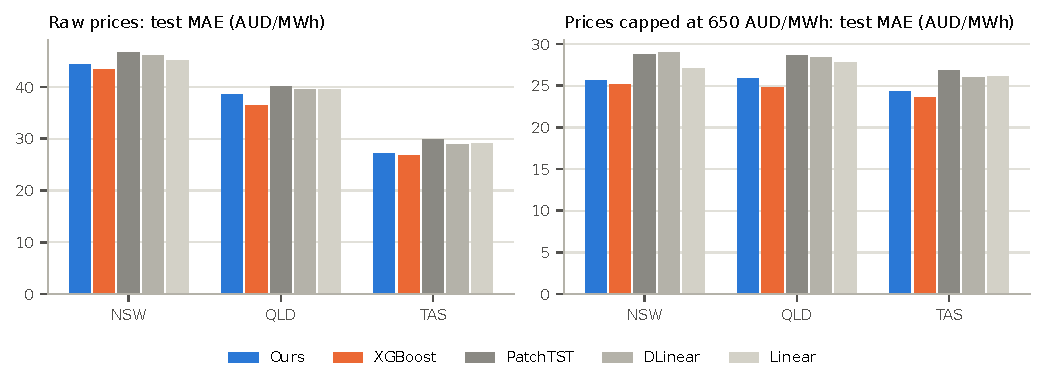
\includegraphics[width=\textwidth]{figures/same_data_comparison.pdf}
\caption{Test MAE per region in the main setting, raw prices (left) and prices capped at 650~AUD/MWh (right); means over three seeds.}
\label{fig:comparison}
\end{figure}

\begin{table}[t]
\centering
\caption{Diebold--Mariano tests, ours minus comparator, in the main setting (negative favours ours). $\Delta$ columns pool the three regions; NSW, QLD and TAS give the raw-price MAE difference per region. MAE averages losses across seeds; CRPS scores seed-averaged quantiles, so its differences need not equal differences between the seed-mean scores in Table~\ref{tab:main}. Newey--West variance uses 48 lags. $^{*}p<0.05$, $^{**}p<0.01$.}
\label{tab:significance}
\resizebox{\textwidth}{!}{% Generated by paper/make_materials.py
\begin{tabular}{lrrrrrrr}
\toprule
& \multicolumn{5}{c}{Raw prices} & \multicolumn{2}{c}{Capped at 650} \\
\cmidrule(lr){2-6}\cmidrule(lr){7-8}
Comparator & $\Delta$MAE & NSW & QLD & TAS & $\Delta$CRPS & $\Delta$MAE & $\Delta$CRPS \\
\midrule
Linear base only & -0.96$^{**}$ & -0.59 & -0.44 & -1.84$^{**}$ & -1.42$^{**}$ & -1.42$^{**}$ & -1.18$^{**}$ \\
XGBoost & +1.11$^{**}$ & +0.93$^{**}$ & +2.10$^{**}$ & +0.31 & +1.11$^{**}$ & +0.75$^{**}$ & +0.31$^{**}$ \\
PatchTST & -2.22$^{**}$ & -2.41$^{**}$ & -1.46$^{**}$ & -2.77$^{**}$ & -0.20 & -2.81$^{**}$ & -1.69$^{**}$ \\
DLinear & -1.57$^{**}$ & -1.82$^{*}$ & -0.97$^{*}$ & -1.91$^{**}$ & +0.58 & -2.53$^{**}$ & -1.46$^{**}$ \\
Linear & -1.28$^{**}$ & -0.89$^{*}$ & -0.93$^{**}$ & -2.03$^{**}$ & +0.53 & -1.72$^{**}$ & -1.49$^{**}$ \\
\bottomrule
\end{tabular}
}
\end{table}

\subsection{When does the decomposition help?}
\label{sec:when}
Fig.~\ref{fig:settings} and Table~\ref{tab:settings} trace every model across three settings, and the first block of Table~\ref{tab:ablations} isolates the dual fields against the same linear base in each.

On the static split (a single fit to 2015--2021), the fields \emph{raise} MAE by 0.92 (raw) and 0.95 (capped) ($p<0.01$), and the dual-field model (41.54) is behind the linear model with the same inputs (40.52). The fields lower the training loss but raise the error on the 2022 validation year: at the selected epoch in NSW1, validation MAE is 60.6 with the fields against 48.6 without. They fit the 2015--2021 level, which shifted in 2022 and again in 2023--2024 (Table~\ref{tab:data}). Normalizing each history window to remove the level did not help, because volatility shifted as well: the median window standard deviation of QLD1 prices is 2.2 times larger in the test period than in training (\ref{app:negative}).

The static-split result is metric-dependent: despite worsening MAE, the fields improve the same base's CRPS (pooled differences $-1.90$ raw and $-1.88$ capped, $p<0.01$, using seed-averaged quantiles). With quarterly refits, pooled MAE differences are not significant ($-0.10$ raw, $-0.06$ capped), while CRPS improves by about 1.1--1.3 ($p<0.01$). Adding predispatch yields pooled gains in MAE ($-0.34$ raw, $p<0.05$; $-0.70$ capped, $p<0.01$) and CRPS ($-1.13$, $-0.94$, $p<0.01$). These are not uniform regional gains: on raw prices, adding the fields changes MAE by $-0.27$ in NSW1 ($p=0.334$), $+0.42$ in QLD1 ($p=0.009$) and $-1.16$ in TAS1 ($p<0.001$). Under capped prices it lowers MAE in all three regions ($p<0.05$). Predispatch lowers every model's three-region mean MAE, and XGBoost's most (39.53 to 35.52 raw), consistent with useful additional information from the operator's dispatch simulation.

\begin{figure}[t]
\centering
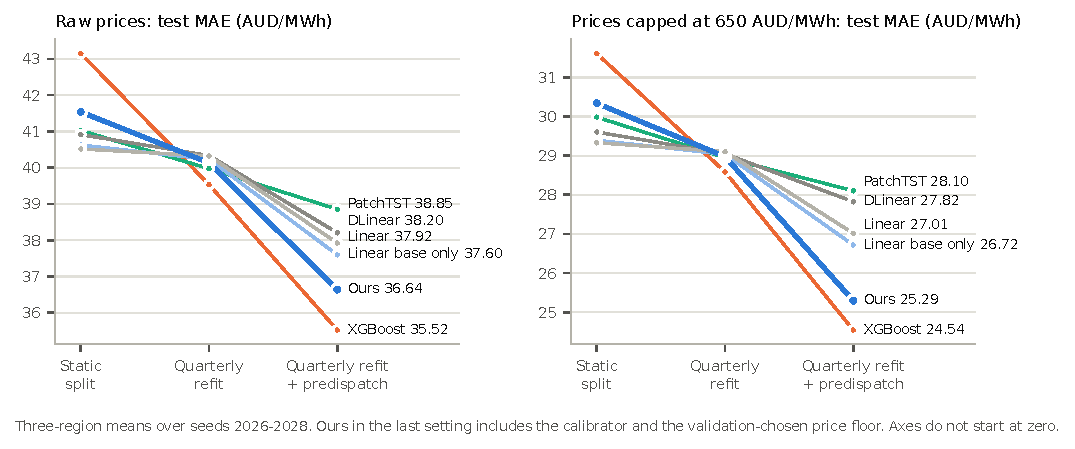
\includegraphics[width=\textwidth]{figures/settings.pdf}
\caption{Three-region mean test MAE of every model in three settings: a single fit on 2015--2021, quarterly refits, and quarterly refits with predispatch. Ours in the last setting includes the calibrator and the price floor. Means over three seeds; axes do not start at zero.}
\label{fig:settings}
\end{figure}

\begin{table}[t]
\centering
\caption{Three-region mean test MAE across settings: static split, quarterly refit, quarterly refit with predispatch (PD). Means over three seeds; best per column in bold.}
\label{tab:settings}
\small
% Generated by paper/make_materials.py
\begin{tabular}{lrrrrrr}
\toprule
& \multicolumn{3}{c}{Raw prices} & \multicolumn{3}{c}{Capped at 650} \\
\cmidrule(lr){2-4}\cmidrule(lr){5-7}
Model & Static & Refit & Refit + PD & Static & Refit & Refit + PD \\
\midrule
Ours & 41.54 & 40.13 & 36.64 & 30.34 & 28.98 & 25.29 \\
Linear base only & 40.62 & 40.23 & 37.60 & 29.39 & 29.04 & 26.72 \\
XGBoost & 43.15 & \textbf{39.53} & \textbf{35.52} & 31.61 & \textbf{28.59} & \textbf{24.54} \\
PatchTST & 41.02 & 39.97 & 38.85 & 29.99 & 28.95 & 28.10 \\
DLinear & 40.91 & 40.33 & 38.20 & 29.61 & 29.05 & 27.82 \\
Linear & \textbf{40.52} & 40.32 & 37.92 & \textbf{29.33} & 29.10 & 27.01 \\
\bottomrule
\end{tabular}

\end{table}

\begin{table}[t]
\centering
\caption{Ablations. Pooled Diebold--Mariano differences (negative is better). The first block compares the dual fields with the same linear base in each setting; each row of the second block is compared with the model it modifies. MAE averages seed losses; CRPS scores seed-averaged quantiles. These pooled tests do not imply improvement in every region. $^{*}p<0.05$, $^{**}p<0.01$.}
\label{tab:ablations}
\small
\resizebox{\textwidth}{!}{% Generated by paper/make_materials.py
\begin{tabular}{lrrrr}
\toprule
& \multicolumn{2}{c}{Raw prices} & \multicolumn{2}{c}{Capped at 650} \\
\cmidrule(lr){2-3}\cmidrule(lr){4-5}
Change & $\Delta$MAE & $\Delta$CRPS & $\Delta$MAE & $\Delta$CRPS \\
\midrule
\multicolumn{5}{l}{\emph{Fields minus linear base}} \\
\quad Static split & +0.92$^{**}$ & -1.90$^{**}$ & +0.95$^{**}$ & -1.88$^{**}$ \\
\quad Quarterly refit & -0.10 & -1.28$^{**}$ & -0.06 & -1.06$^{**}$ \\
\quad Quarterly refit + predispatch & -0.34$^{*}$ & -1.13$^{**}$ & -0.70$^{**}$ & -0.94$^{**}$ \\
\multicolumn{5}{l}{\emph{Added to fields + predispatch}} \\
\quad Hinge features on predispatch price & -0.25$^{**}$ & -0.95$^{*}$ & -0.39$^{**}$ & -0.26$^{**}$ \\
\quad Calibrator & -0.31$^{*}$ & -0.26$^{*}$ & -0.44$^{**}$ & -0.22$^{**}$ \\
\quad Price floor (after calibrator) & -0.31$^{**}$ & -0.03$^{**}$ & -0.29$^{**}$ & -0.01 \\
\quad Interconnector inputs (after floor) & +0.04 & +0.04 & +0.19$^{**}$ & -0.04 \\
\bottomrule
\end{tabular}
}
\end{table}

\subsection{Diagnosis and corrections}
\label{sec:diagnosis}
To locate the remaining gap to XGBoost, we split the absolute-error difference by condition for the calibrated model before applying the lower bound. In QLD1, its seed-mean MAE gap is 2.9~AUD/MWh; for the seed-averaged point forecasts used in this diagnosis, the gap is 2.31 (38.56 against 36.25). Hours with a non-positive actual price (13\% of hours) account for 47\% of the latter gap, and hours in the lowest net-load quintile, largely the same midday solar hours, for 48\%. The calibrated model forecast prices below $-100$~AUD/MWh in 0.23\% of hours, against 0.01\% of actual prices and none for XGBoost: the 3.2\% of hours in which it forecast below $-50$ carry 31\% of the gap. Linear heads extrapolate in asinh space, and the inverse transform can turn modest transformed-space deviations into deep negative prices. The fitted XGBoost comparator did not exhibit these extrapolations; this observation is not a general range-preservation guarantee for boosted trees.

Two corrections follow (second block of Table~\ref{tab:ablations}). Letting the model respond nonlinearly to predispatch, by hinge features of the predispatch price or by the calibrator, lowers MAE by 0.25--0.44 ($p<0.01$ except the raw calibrator, $p<0.05$); the calibrator is retained because it also gives the best tail scores. The validation-chosen price floor lowers MAE by a further 0.31 (raw) and 0.29 (capped), significantly in every region and most in QLD1 ($-0.82$ raw). In QLD1 the chosen point floors are $-37$ to $-48$~AUD/MWh in seven of the eight refits. Adding predispatch interconnector flows and limits does not help ($+0.04$ raw, $+0.19$ capped): the predispatch price already reflects the network constraints.

\subsection{Price tails}
Table~\ref{tab:tails} scores the tails. On negative-price hours, our final model has lower CRPS and 0.05-quantile pinball loss than all five comparators in that table under both price treatments, significantly lower in the pooled tests including against XGBoost (raw CRPS 14.52 against 15.96; $p<0.001$). This does not establish superiority to every development variant: the calibrator without the lower bound achieves raw negative-price CRPS 14.17 and lower-tail pinball loss 4.30, compared with 14.52 and 4.74 after clipping. Capped negative-price CRPS likewise changes from 13.99 to 14.28. The lower bound therefore trades some tail accuracy for lower overall MAE. On capped prices the final model has the lowest spike-hour CRPS in the table (121.1 against 138.3 for XGBoost; $p<0.01$); its difference to PatchTST is not significant, and PatchTST has slightly lower upper-tail pinball loss. On raw spike hours its CRPS difference to XGBoost is not significant, while it is worse than PatchTST, DLinear and the linear model ($p<0.05$).

\begin{table}[t]
\centering
\caption{Probabilistic scores in the price tails, main setting, mean of the three regions, scoring seed-averaged quantiles. Lower is better for losses; best among the displayed models is bold. Coverage is evaluated over all test hours. $^{\dagger}$/$^{\ddagger}$: ours is significantly better/worse than that model in a pooled Diebold--Mariano test on per-origin event-hour losses ($p<0.05$). Point estimates average event-hour losses within each region; tests first average within each origin, so their differences use a different weighting.}
\label{tab:tails}
\resizebox{\textwidth}{!}{% Generated by paper/make_materials.py
\begin{tabular}{lrrrrr}
\toprule
& \multicolumn{2}{c}{Negative-price hours} & \multicolumn{2}{c}{Spike hours ($>$300)} & \\
\cmidrule(lr){2-3}\cmidrule(lr){4-5}
Model & CRPS & $q_{0.05}$ pinball & CRPS & $q_{0.95}$ pinball & 90\% coverage \\
\midrule
\multicolumn{6}{l}{\emph{Raw prices}} \\
Ours & \textbf{14.52} & \textbf{4.74} & 800.3 & 675.3 & 91.5\% \\
Linear base only & 16.21$^{\dagger}$ & 5.82$^{\dagger}$ & 882.3$^{\dagger}$ & 777.2$^{\dagger}$ & 93.1\% \\
XGBoost & 15.96$^{\dagger}$ & 6.13$^{\dagger}$ & 790.5 & 640.3 & 87.7\% \\
PatchTST & 17.99$^{\dagger}$ & 7.51$^{\dagger}$ & 745.2$^{\ddagger}$ & 600.3$^{\ddagger}$ & 90.0\% \\
DLinear & 17.25$^{\dagger}$ & 7.33$^{\dagger}$ & \textbf{740.3}$^{\ddagger}$ & \textbf{591.7}$^{\ddagger}$ & 89.1\% \\
Linear & 17.25$^{\dagger}$ & 7.38$^{\dagger}$ & 741.8$^{\ddagger}$ & 593.8$^{\ddagger}$ & 89.0\% \\
\midrule
\multicolumn{6}{l}{\emph{Capped at 650}} \\
Ours & \textbf{14.28} & \textbf{4.83} & \textbf{121.1} & 77.2 & 90.5\% \\
Linear base only & 16.23$^{\dagger}$ & 6.07$^{\dagger}$ & 146.7$^{\dagger}$ & 87.5$^{\dagger}$ & 92.4\% \\
XGBoost & 15.47$^{\dagger}$ & 6.13$^{\dagger}$ & 138.3$^{\dagger}$ & 91.0$^{\dagger}$ & 86.2\% \\
PatchTST & 17.90$^{\dagger}$ & 7.42$^{\dagger}$ & 127.8 & \textbf{77.0} & 90.0\% \\
DLinear & 17.19$^{\dagger}$ & 7.32$^{\dagger}$ & 141.7$^{\dagger}$ & 85.5 & 89.0\% \\
Linear & 17.31$^{\dagger}$ & 7.44$^{\dagger}$ & 141.9$^{\dagger}$ & 85.5 & 88.7\% \\
\bottomrule
\end{tabular}
}
\end{table}

\subsection{Case studies}
Fig.~\ref{fig:cases} shows two test days chosen by fixed rules. On the QLD1 day with the lowest mean price (1 October 2023), the linear base and the dual fields keep the midday forecast positive; the calibrator brings it into negative prices but overshoots to about $-85$~AUD/MWh, and the floor ($-43$) clips the overshoot. The day's MAE is 12.2 for our model, 14.1 for XGBoost and 17.3 for predispatch. On the NSW1 day on which predispatch most overstated the peak (24 October 2024, predispatch 17{,}500~AUD/MWh against an actual price below 300), every model is pulled up at 17:00; ours reaches about 470 and XGBoost about 280 (day MAE 57.1 and 52.8). Such phantom spikes remain a failure mode.

\begin{figure}[t]
\centering
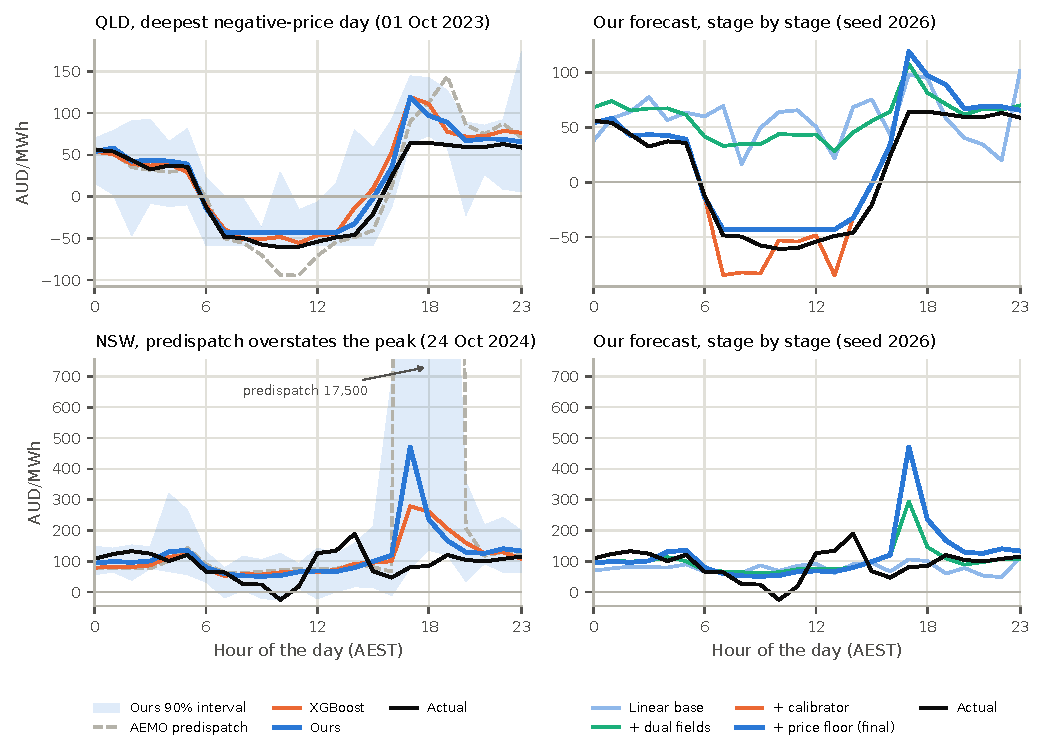
\includegraphics[width=\textwidth]{figures/cases.pdf}
\caption{Case studies, chosen by fixed rules on the test split. Top: QLD1 day with the lowest mean price. Bottom: NSW1 day on which predispatch most overstated the peak (forecast above 1{,}000, actual below 300~AUD/MWh). Left: our forecast with its 90\% interval, XGBoost, predispatch and the actual price. Right: cumulative component outputs of the same jointly trained seed-2026 model, not independently retrained ablations. On the NSW1 day the lower bound is not binding, so the calibrated and final forecasts coincide.}
\label{fig:cases}
\end{figure}

\subsection{Computational cost}
Table~\ref{tab:cost} reports the size of each model and the wall-clock time of one quarterly refit (NSW1, 2023Q3 test quarter, seed 2026) on one GPU. Every model refits in four to six minutes; the dual-field model costs about 20\% more than its linear base and less than PatchTST. A full evaluation (eight refits, three regions, three seeds) takes a few hours per model on one GPU.

\begin{table}[t]
\centering
\caption{Model size and wall-clock time of one quarterly refit (NSW1, 2023Q3, seed 2026), each run alone on an NVIDIA L40 shared with other users; times are indicative. XGBoost size is the total number of boosting rounds over the 24 per-hour models; Linear base only keeps the field modules, which are still fitted by the decomposition loss.}
\label{tab:cost}
\small
% Generated by paper/make_materials.py
\begin{tabular}{lrr}
\toprule
Model & Parameters & Seconds per refit \\
\midrule
Ours & 277,747 & 312 \\
Linear base only & 275,629 & 258 \\
XGBoost & 2,871 rounds & 269 \\
PatchTST & 599,730 & 364 \\
DLinear & 78,120 & 252 \\
Linear & 83,232 & 237 \\
\bottomrule
\end{tabular}

\end{table}

%% ---------------------------------------------------------------------------
\section{Discussion}
\label{sec:discussion}

\paragraph{Why decomposition has mixed value on a static split} The identity $c+e+r=x$ means the fields introduce no new observations, but their nonlinear representation can express relationships unavailable to a single linear map. In our static-split experiments this added structure worsens MAE while improving the same base's CRPS. Lower training loss and higher validation MAE are consistent with sensitivity to the changing price regime; they do not isolate regime shift as the sole cause. Informer also performs poorly in the static screening (\ref{app:negative}), but differences in normalization alone do not establish the cause of that result.

\paragraph{Value of recalibration and predispatch} Refitting incorporates more recent observations, and predispatch supplies the operator's forward-looking assessment of offers, demand and constraints. The pooled ablations support combining these inputs with the dual-field residual, but raw-price MAE gains from the fields are concentrated in TAS1 and do not extend to QLD1. Negative-price scores improve over the main-table baselines for the complete model; those gains cannot be attributed to the decomposition alone, because the calibrator and lower bound also change its forecasts.

\paragraph{The gap to XGBoost} XGBoost uses these inputs more accurately on average, and its fitted predictions avoid the extreme negative extrapolations observed in the neural model. The calibrator and lower bound recover part of the gap, but XGBoost remains ahead in the 100--300~AUD/MWh band and in QLD1. For overall MAE on this benchmark, XGBoost is the stronger choice. The dual-field model offers better negative-price scores than the main-table baselines, while the unbounded calibrator variant offers still better negative-price scores. Whether either improves storage or demand-response decisions requires a separate decision-based evaluation.

\paragraph{Limitations} The study covers three regions of one market and a two-year test period. The empirical lower bound is selected on validation data, but the decision to introduce it followed a diagnosis of test-period errors; these results should therefore be confirmed on a later untouched period. On raw spike hours the model is behind the linear baselines, and its regional gains are heterogeneous. Predispatch run history is missing for October 2022, and its horizon does not always cover all 24 target hours. The hard event-activity penalty has no training gradient. Tail tests drop origins without events, so their 48 lags count retained origins rather than fixed elapsed hours; reported significance is conditional on that weighting and dependence approximation. Hyperparameters were developed on the static split and were not re-tuned for the recalibrated setting.

%% ---------------------------------------------------------------------------
\section{Conclusion}
\label{sec:conclusion}

The value of trend--event decomposition in rolling electricity price forecasting depends on the metric, region and recalibration setting. On the static split, adding the fields worsens the same linear base's MAE but improves its CRPS. With quarterly refits and predispatch inputs, pooled MAE and CRPS improve, although raw-price MAE still worsens in QLD1. The complete model, including the calibrator and empirical lower bound, improves MAE over PatchTST, DLinear and a linear baseline and improves negative-price scores over all five main-table comparators. The lower bound sacrifices some negative-price accuracy relative to the unbounded calibrator. XGBoost retains the lowest overall MAE and CRPS. Future work should test these tradeoffs on an untouched period and in other markets, and model predispatch errors explicitly to handle phantom spikes.

%% ---------------------------------------------------------------------------
\section*{CRediT authorship contribution statement}
\textbf{zl:} Conceptualization, Methodology, Software, Validation, Formal analysis, Investigation, Data curation, Writing -- original draft, Writing -- review \& editing, Visualization.

\section*{Declaration of competing interest}
The authors declare that they have no known competing financial interests or personal relationships that could have appeared to influence the work reported in this paper.

\section*{Declaration of generative AI and AI-assisted technologies in the manuscript preparation process}
%% To be confirmed and completed by the author before submission.
During the preparation of this work the author(s) used [tool name] in order to [purpose]. After using this tool, the author(s) reviewed and edited the content as needed and take(s) full responsibility for the content of the published article.

\section*{Data availability}
All data are public and were obtained from the Australian Energy Market Operator \citep{aemo2025priceanddemand,aemo2025mmsdm,aemo2025dwgm}. Code and configurations that reproduce the results will be made available.

%% ---------------------------------------------------------------------------
\appendix

\section{Field separation and static-split development}
\label{app:static}

In our forecasting transplant, the original Gabor DGF with globally learned positions carries little of the historical spike signal, while the CTF absorbs it. We quantify this by $R_e=\operatorname{mean}_{\mathcal S}e^{(1)}/\operatorname{mean}_{\mathcal S}x^{(1)}$, where $\mathcal S$ contains historical positions with raw price above 300~AUD/MWh across all test windows. Both numerator and denominator are in standardized asinh space, and repeated positions in overlapping windows are retained. The ratio is $-0.04$ to $0.00$ for the Gabor DGF and 0.28 to 0.33 for detected events (Fig.~\ref{fig:field-separation}, Table~\ref{tab:field-separation}). It is a transformed-signal diagnostic, not a fraction of monetary price or explained variance. Fig.~\ref{fig:ladder} shows the static-split development, where most MAE improvement came from target transformation and fundamental inputs. Table~\ref{tab:ablations-static} reports the structural and detector ablations: suppression and the median level matter, while event count and threshold have smaller effects.

\begin{figure}[t]
\centering
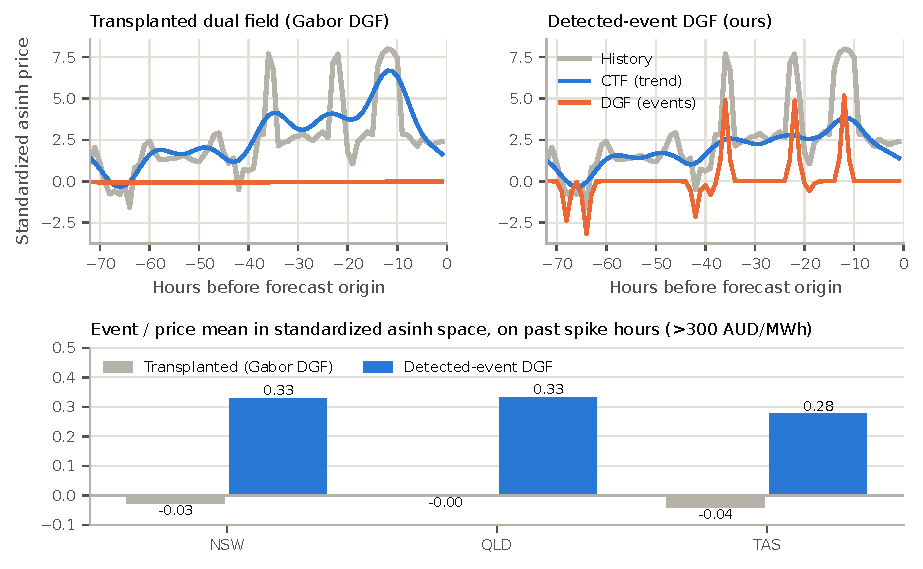
\includegraphics[width=\textwidth]{figures/field_separation.pdf}
\caption{Field separation. Top: one NSW1 test window in standardized asinh price; the Gabor DGF stays near zero (left), whereas detected events capture localized deviations (right). Bottom: event-to-price mean ratio $R_e$ in standardized asinh space, restricted to historical raw-price spikes above 300~AUD/MWh. This is not a monetary contribution share.}
\label{fig:field-separation}
\end{figure}

\begin{table}[t]
\centering
\caption{Event-to-price mean ratio $R_e$ on historical spike positions in test windows, measured in standardized asinh space.}
\label{tab:field-separation}
\small
% Generated by paper/make_materials.py
\begin{tabular}{lrrr}
\toprule
Event field & NSW & QLD & TAS \\
\midrule
Transplanted (Gabor) & -0.03 & -0.00 & -0.04 \\
Detected events (ours) & 0.33 & 0.33 & 0.28 \\
\bottomrule
\end{tabular}

\end{table}

\begin{figure}[t]
\centering
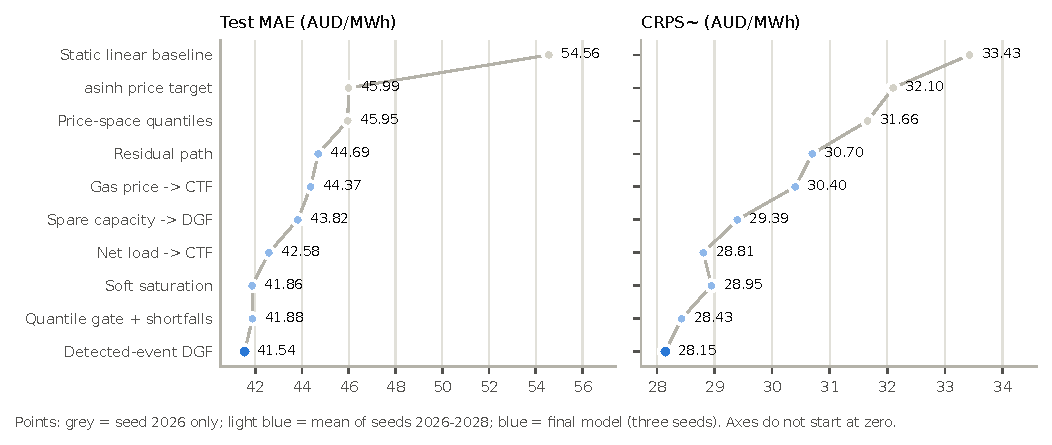
\includegraphics[width=\textwidth]{figures/ablation_ladder.pdf}
\caption{Development on the static split: three-region mean test MAE and CRPS on raw prices; each step changes one component. Grey: seed 2026 only; blue: means over seeds 2026--2028. Axes do not start at zero.}
\label{fig:ladder}
\end{figure}

\begin{table}[t]
\centering
\caption{Structural and detector ablations of the detected-event DGF on the static split, raw prices, three-region means over three seeds (MAE $\pm$ seed standard deviation). The last column gives the paired MAE difference to the detected-event DGF per seed; positive means the variant is worse.}
\label{tab:ablations-static}
\resizebox{\textwidth}{!}{% Generated by paper/make_materials.py
\begin{tabular}{lrrrr}
\toprule
Variant & MAE & Window RMSE & CRPS & $\Delta$MAE vs detected (seeds) \\
\midrule
\multicolumn{5}{l}{\emph{Structure}} \\
Transplanted dual field (Gabor DGF) & 41.88 $\pm$ 0.22 & 79.21 & 28.43 & +0.38 / +0.03 / +0.58 \\
No decomposition (heads read raw history) & 41.90 $\pm$ 0.11 & 79.31 & 28.40 & +0.30 / +0.25 / +0.51 \\
Adaptive attention atoms + echo & 41.84 $\pm$ 0.05 & 79.01 & 28.09 & +0.30 / +0.28 / +0.30 \\
Detected events + daily echo & 42.21 $\pm$ 0.11 & 79.93 & 28.22 & +0.79 / +0.47 / +0.73 \\
Detected-event DGF & 41.54 $\pm$ 0.06 & 78.80 & 28.15 & -- \\
\midrule
\multicolumn{5}{l}{\emph{Detector settings (8 events, 3-hour separation, learned threshold, median)}} \\
4 events & 41.65 $\pm$ 0.03 & 78.85 & 28.25 & +0.13 / +0.01 / +0.18 \\
16 events & 41.50 $\pm$ 0.08 & 78.76 & 28.15 & -0.08 / -0.03 / -0.03 \\
No suppression (1-hour separation) & 41.85 $\pm$ 0.03 & 79.00 & 28.05 & +0.36 / +0.21 / +0.35 \\
6-hour separation & 41.51 $\pm$ 0.05 & 78.77 & 28.28 & -0.05 / -0.11 / +0.05 \\
No threshold & 41.63 $\pm$ 0.08 & 78.98 & 27.97 & +0.21 / -0.03 / +0.07 \\
Mean baseline & 41.64 $\pm$ 0.03 & 78.91 & 28.02 & +0.09 / +0.05 / +0.15 \\
\bottomrule
\end{tabular}
}
\end{table}

\section{Designs that did not help}
\label{app:negative}

The following were tested with three seeds and are reported for completeness (full records are in the code repository).
\begin{itemize}
\item \emph{Window-normalized fields} on the linear base, with the residual rescaled by the window's price scale: raw MAE 44.29 against 41.54 unnormalized (static split), because test-period volatility is about twice the training volatility.
\item \emph{Fields on the quantiles only}, with asinh-space quantiles and the point forecast from the linear base: the fields widened the 90\% interval from 171 to 418~AUD/MWh and raised CRPS from 28.94 to 31.25 (static split).
\item \emph{A future event field}, a three-component mixture for spike and trough probabilities, did not beat a logistic regression on the same inputs in precision--recall.
\item \emph{iTransformer and Informer} (static split, raw MAE 43.20 and 46.65) were less accurate than PatchTST (41.02) and DLinear (40.91); Informer's validation loss was lowest after one to five epochs.
\item \emph{Predispatch interconnector inputs}: no gain (Section~\ref{sec:diagnosis}).
\end{itemize}

\clearpage
\bibliographystyle{elsarticle-num-names}
\bibliography{references}

\end{document}
